\textbf {Kernel methods}\\

In the multidimensional case we are limited to polynomial type regressions due to the curse of dimensionality, so we use kernel methods, in particular the Gaussian kernel.\\
Use two hyperparameters:
\begin{itemize}
	\item $\lambda$ that regularize the solution $\rightarrow$ allows you to find a model that is smooth
	\item the 3 hyperparameters of the kernel, in this case only the gamma is taken into account: a parameter that regulates the no linearity of the solution
\end{itemize}
there are combinations of $\lambda$ and gamma that more or less lead to the same solution. So $\lambda$ and $\gamma$ are parameters that are not completely disconnected, you can find more or less the usual models with different values of these quantities.\\
How to find the best $\lambda$ and $\gamma$ values:\\
We find best values of hyperparmeters through validation procedure (split the data, create the model with part of the data, and test the quality of hyperparmeters on a set of data that are not used during the model creation), the best combination of hypers is the one that minimize the error on the validation set( $\rightarrow$ the set of data not used for creating the model)
The best thing to do is to mediate the results.\\
The splitting of data should not be done only once, but should be repeated because with a single report the variance is higher, but if you take the average I'm more confident that my estimator is close to the real average.\\
Observation: the loop on $k$ is put as the first loop in our implementation (putting it inside I could avoid keeping the array of all errors) because my estimate with $k$ inside would be subject to 2 types of variance: a variance due to the estimator same that can not be eliminated, the other is the variance of how the learning set and the validation set occur. Risk of selecting bad $\lambda$ and $\gamma$ because my solution is determined by the variance of the quality of the splitting. Writing the code as we wrote it, the splitting part is always the same for every $\gamma$ and $\lambda$ and this reduces the variance of my estimator.\\
Last observation: The graph, even increasing range, does not pass from all points because of the 64-bit precision that is not able to reach them all.

\begin{figure}
	\centering
	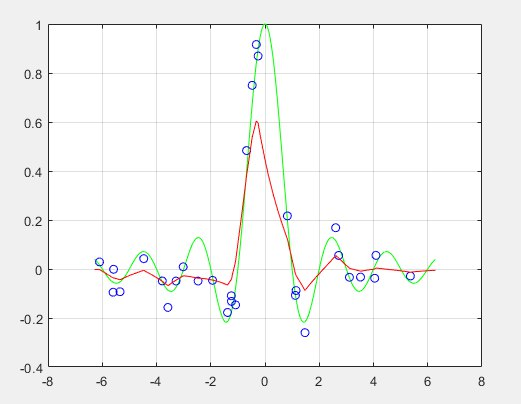
\includegraphics[width=0.5\textwidth]{kml1g1.png}
	\caption{$\lambda$ = 1 $\gamma$ = 1}
%	\label{fig:$\lambda$ = 1 $\gamma$ = 1}

\end{figure}
\begin{figure}
Less smoothness\\

	\centering
	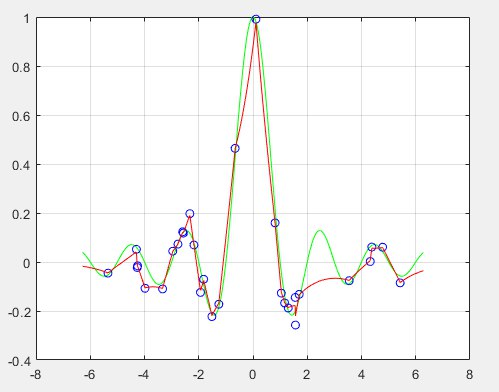
\includegraphics[width=0.5\textwidth]{kml1g001.png}
	\caption{$\lambda$ = 0,01 $\gamma$ = 1}
%	\label{fig:\lambda = 0,01 \gamma = 1}

\end{figure}
\begin{figure}
More smoothness\\

	\centering
	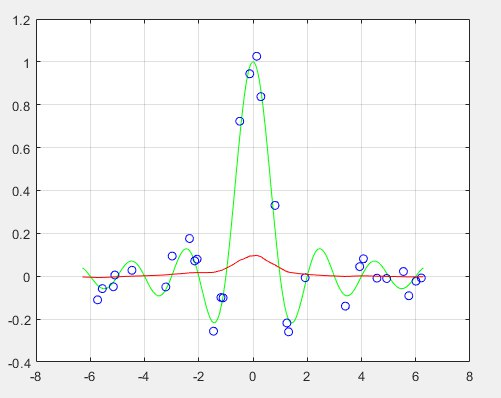
\includegraphics[width=0.5\textwidth]{kml1g25.png}
	\caption{$\lambda$ = 25 $\gamma$ = 1}
%	\label{fig:\lambda = 25 \gamma = 1}

\end{figure}
\begin{figure}
More non linearity\\

	
	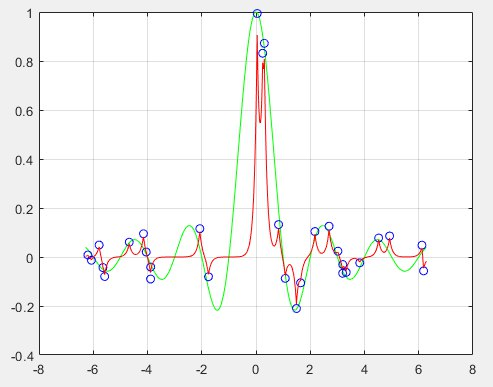
\includegraphics[width=0.5\textwidth]{kml10g01.png}
	\centering
	\caption{$\lambda$ = 0,1 $\gamma$ = 10}
%	\label{fig:\lambda = 0,1 \gamma = 10}
\end{figure}

\begin{figure}
	
Very irregular and non-linear, it can not reach all the points anyway due to the precision of the machine.\\

	
	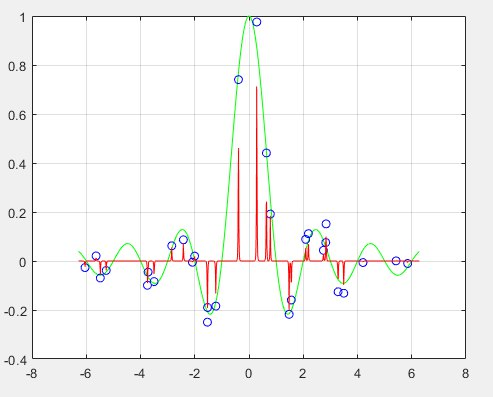
\includegraphics[width=0.5\textwidth]{kml100g0.png}
	\centering
	\caption{$\lambda$ = 0 $\gamma$ = 100}
%	\label{fig:\lambda = 0 \gamma = 100}
\end{figure}


